\documentclass{article}
\usepackage{amsmath,amsthm,amssymb}
\usepackage{bm}
\usepackage{graphicx}
\usepackage[margin=1in]{geometry}
\newcommand{\uvecr}{{\bm{\hat{\textnormal{\bfseries r}}}}}
\DeclareRobustCommand{\uvec}[1]{{%
		\ifcat\relax\noexpand#1%
		% it should be a Greek letter
		\bm{\hat{#1}}%
		\else
		\ifcsname uvec#1\endcsname
		\csname uvec#1\endcsname
		\else
		\bm{\hat{\mathbf{#1}}}%
		\fi
		\fi
}}
\begin{document}

\textbf{Name:} Joe

\textbf{Date:} 26/10/22

\bigskip

We need to calculate the structure factor of the system. This can calculated by finding the Fourier Transform of the order parameter $\phi$ and then finding $\langle \phi(\boldsymbol{k})\phi(\boldsymbol{-k})\rangle$, or $\langle \phi(\boldsymbol{k})\phi(\boldsymbol{k}+\boldsymbol{k_{0}})\rangle$ for some Fourier space element $k_{0}$ (basically the Fourier analogue of calculating the Correlation Function $\langle\phi(\boldsymbol{x})\phi(\boldsymbol{x}+\boldsymbol{r})\rangle$, where $\boldsymbol{k_{0}}$ and $\boldsymbol{r}$ are arbitrary vectors in Fourier and real space). I'm not clear on which equation to use.

\medskip

Once we have the structure factor S, we can plot it against $k$ for various times $t$, and we'll find that they produce different decay curves. For larger $t$, we'll find that the decay curve is steeper. If we scale the $k$ axis by $t^{1/2}$ or $t^{-1/2}$ (I'm not sure which yet), all the curves will fall onto each other.



From this, we should be able to extract the dynamic scaling exponent, which has a value of $z=2$.

\medskip

$\nabla\phi$ can discretised along a square grid with separation $\Delta x$ in each direction.

\begin{equation}\label{discretized laplacian}
	\nabla^2 \phi \approx \frac{\Delta \phi}{\Delta x^{2}} = \frac{\phi_{i+1,j} + \phi{i-1,j} + \phi{i,j+1} + \phi{i,j-1}-4\phi}{\Delta x^{2}}
\end{equation}

\medskip

Also check out "Granular Media.pdf", which is the "PRL 3" article on the Moodle page. Also look at "Growth Laws" in Bray's paper (not sure if section 2.5 or section 7, try both).

\medskip

\rule{\textwidth}{0.4pt}

\textbf{Name:} Joe

\textbf{Date:} 27/10/22

\bigskip

I've spent some time coding the basic diffusion equation:

\begin{equation}\label{diffusion equation}
	\frac{\partial \phi}{\partial t} = \nabla^{2} \phi
\end{equation}

Using equation \ref{discretized laplacian} to discretize the Laplacian operator. It was vectorised using the following logic.

\medskip

We can write the order parameter as some vector $\boldsymbol{\phi}$. Suppose we look at a 3$\times$3 lattice:

\begin{equation}
	\boldsymbol{\phi} = \begin{pmatrix}
	\phi_{00} & \phi_{01} & \phi_{02}\\
	\phi_{10} & \phi_{11} & \phi_{12}\\
	\phi_{20} & \phi_{21} & \phi_{22}
	\end{pmatrix}
\end{equation}

We argue that for periodic boundary conditions, when considering a term for the Laplacian such as $\phi_{i+1,j}$, when $i=2$, $i+1=0$. Conversely, for $\phi_{i-1,j}$, when $i=0$, $i-1=2$.

The \texttt{Numpy} function \texttt{numpy.roll} enables us to move elements in a matrix with ease. To move each row one row down, including moving the bottom row to the top, we type:

\begin{verbatim}
	np.roll(phi, N)
\end{verbatim}

Where \texttt{N} is the length of a row or column (in this case, \texttt{N}=3). To move one column over, we type:

\begin{verbatim}
np.roll(phi, 1, axis=1)
\end{verbatim}

This is given a little more detail in the Github file \texttt{RollingMatrices.py}.

\medskip

When we discretize equation \ref{diffusion equation}, we can solve it using \texttt{Scipy}'s \texttt{odeint} function from its \texttt{Integrate} module. Since \texttt{odeint} only accepts one-dimensional inputs, we can reshape the $\boldsymbol{\phi}$ lattice into an \texttt{N}$^{2}$ long array and give it to \texttt{odeint}. Then, we can use \texttt{numpy.roll} on the lattice and perform all the discretized Laplacian calculations in one matrix. We then reshape the lattice again to make it more palatable for \texttt{odeint} and it repeats this process.

\medskip

After \texttt{odeint} has given us the solution, we can retrieve the lattice by reshaping each row of the solution array. Currently, this is done using a for loop, which isn't really ideal, but I'm not sure how to vectorise it yet.

Then, again using for loops because vectorising things is difficult, we can retrieve $\phi$ for a given lattice site for every point in time. This gives the plot in figure \ref{first phi plot}.

\begin{figure}
	\centering
	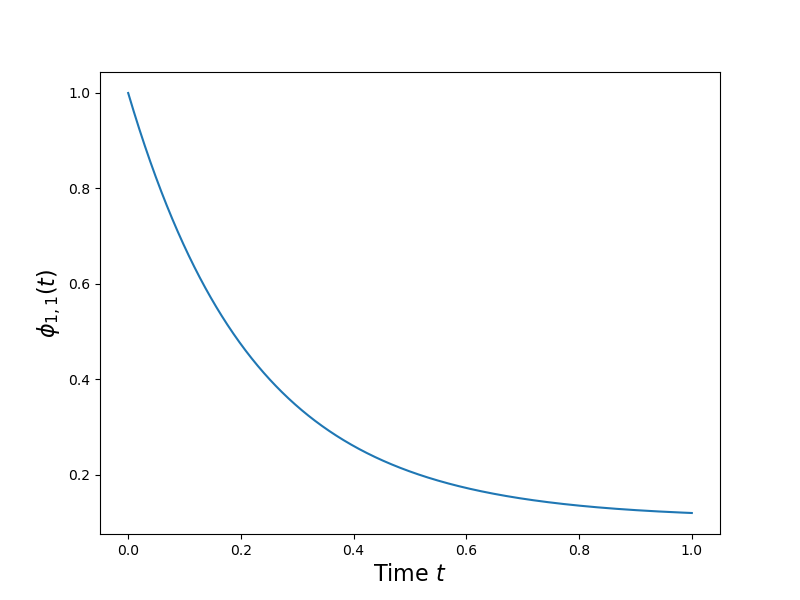
\includegraphics[width=0.8\textwidth]{phi_plot.png}
	\caption{\label{first phi plot}Plotting $\phi_{1,1}$, which was initialised to have the value $\phi=1$, against time $t$. It displays exponential decay behaviour, which is what we expect.}
\end{figure}

Since $\phi$ decays exponentially here, we could use some \texttt{SciPy} curve fitting to find decay constants, although I don't think this will be as important when we include a potential, as we're required to.

\medskip

We'll need to animate this to make what's happening a lot clearer. This graph works great for a single lattice site, but it's not any good for the whole lattice. I remember Moriarty had some things written on animations.

\medskip

This little bit is a little while (~2 hours) after the previous section of this diary entry. I've pulled together a rudimentary animation, although I suspect that the calculations are wrong. Figure \ref{phi after 1 second} shows the lattice after 1 second (after the system has evolved in time). The lattice sites around the centre, which is initialised to have value 1, do not evenly "grow" in value.

\begin{figure}
	\centering
	\includegraphics[width=0.8\textwidth]{first_evolution.png}
	\caption{\label{first phi plot}Plotting $\phi_{1,1}$, which was initialised to have the value $\phi=1$, against time $t$. It displays exponential decay behaviour, which is what we expect.}
\end{figure}

\end{document}
